\section{Auswertung}

\subsection{Eckige Stäbe, einseitige Einspannung}

Um den Elastizitätsmodul von den eckigen Stäben bei einseitiger Einspannung zu bestimmen wird zunächst eine Grafik erstellt. Dafür wird die Gesamtauslenkung der eckigen Stäbe bei einseitiger Einspannung D(x) aus den Tabellen \ref{tab:1} und \ref{tab:2} gegen $Lx^2-\frac{x^3}{3}$ aufgetragen. Dabei enstehen folgende Diagramme:

\begin{figure}[H]
    \centering
    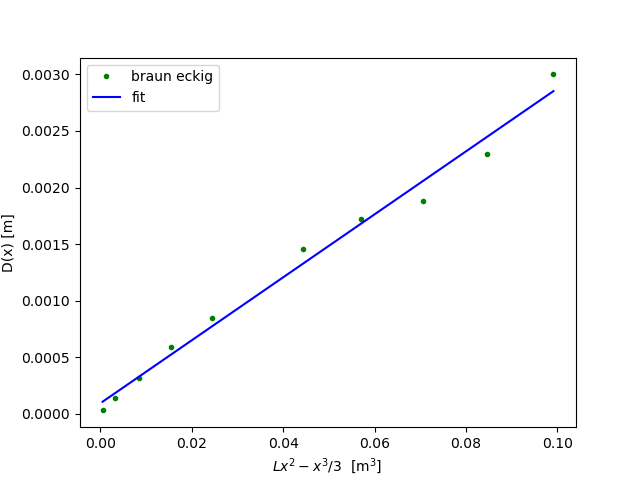
\includegraphics{bee.png}
    \captionof{figure}{Biegung eines braunen, eckigen Stabes mit zugehöriger Ausgleichsrechnung, bei einseitiger Einspannung.}
\end{figure}

\begin{figure}[H]
    \centering
    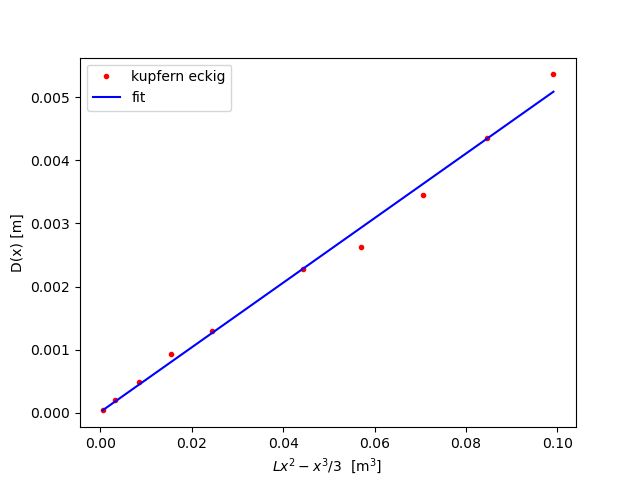
\includegraphics{kee.png}
    \captionof{figure}{Biegung eines kupfernen, eckigen Stabes mit zugehöriger Ausgleichsrechnung, bei einseitiger Einspannung.}
\end{figure}

Die Ausgleichsrechnungen wurden mit der allgemeinen Geradengleichung: $y = ax+b$ durchgeführt.
Aus diesen Graphen und den Ausgleichsrechnungen lässt sich der Elastizitätsmodul mit folgender Formel berechnen:

\begin{align*}
    E = \frac{m*g}{2*I*a}
\end{align*}

Dabei ist a die mit der Ausgleichsrechnung bestimmte Steigung der Ausgleichsgeraden. Die Masse m beträgt hier jeweils 1.0543kg.
I ist das Flächenträgheitsmoment. Da die Stäbe Quadratisch sind, ist das Flächenträgheitsmoment: $I=\frac{h^4}{12}$.
Beide Stäbe haben als Kantenlänge h=1cm. Die berechneten Steigungen sind:

\begin{align*}
    a_{braun} = (2.78\pm 0.11) \frac{10^{-2}}{m^2}\\
    a_{kupfern} = (5.1\pm 0.16) \frac{10^{-2}}{m^2} 
\end{align*}

Mit diesen Werten ergibt sich für die Elastizitätsmodule:
\begin{align*}
    E_{braun} = (223\pm 9) GPa \\
    E_{kupfern} = (1.22\pm 4) GPa
\end{align*}

\subsection{runde Stäbe, einseitige Einspannung}

Für die runden Stäbe ist das Vorgehen identisch zu dem Vorgehen bei den Eckigen. Hier werden die Werte von D(x) aus \ref{tab:3} und \ref{tab:4} genommen. Diese werden genauso gegen $Lx^2-\frac{x^3}{3}$ aufgetragen. Dabei entstehen folgende Diagramme:

\begin{figure}[H]
    \centering
    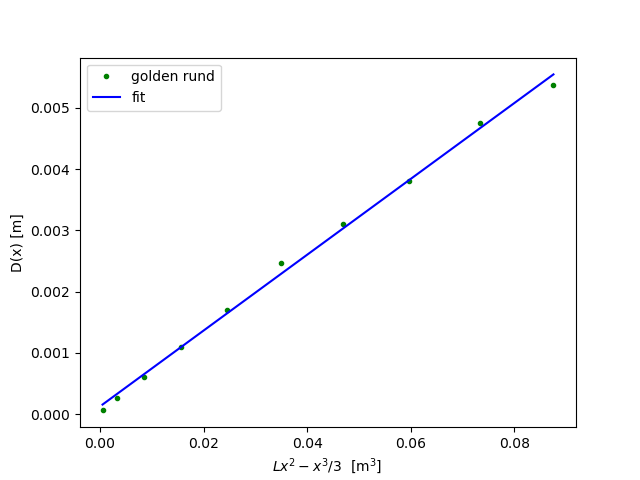
\includegraphics{gre.png}
    \captionof{figure}{Biegung eines goldenen, runden Stabes mit zugehöriger Ausgleichsrechnung, bei einseitiger Einspannung.}
\end{figure}

\begin{figure}[H]
    \centering
    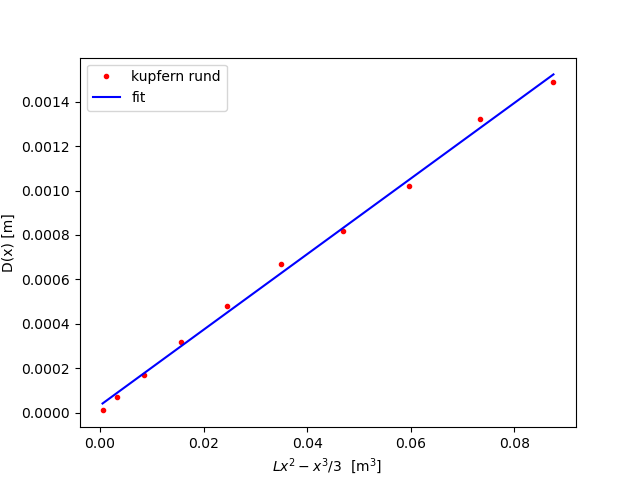
\includegraphics{kre.png}
    \captionof{figure}{Biegung eines kupfernen, runden Stabes mit zugehöriger Ausgleichsrechnung, bei einseitiger Einspannung.}
\end{figure}

Auch die Formel für den Elastizitätsmodul bleibt gleich. Die einzigen Unterschiede sind hier das Flächenträgheitsmoment und die an den Stab gehängte Masse. Die Masse beträgt 0.2492kg für den kupfernen Stab und 0.552kg für den Messingstab. Das Flächenträgheitsmoment lässt sich aufgrund des runden Querschnitts nun folgendermaßen bestimmen:

\begin{align*}
    \frac{\pi R^4}{4}
\end{align*}

Der Durchmesser der beiden Stäbe beträgt 1cm.

Nun lassen sich wieder die Elastizitätsmodule bestimmen:

\begin{align*}
    E_{kupfern} = (146.5\pm 2.6) GPa \\
    E_{golden} = (89\pm 17) GPa 
\end{align*}

\subsection{eckige Stäbe, beidseitige Einspannung}

Für die eckigen Stäbe bei beidseitiger Einspannung werden Werte für D(x) aus \ref{tab:1} und \ref{tab:2} in Diagrammen aufgetragen. Dabei werden jeweils die Werte links vom Aufhängungspunkt (27.5cm) und rechts vom Aufhängungspunkt gesondert aufgetragen. Die Werte links vom Aufhängungspunkt werden dabei gegen $3L^2x-4x^3$ und die Werte rechts vom Aufhängungspunkt gegen $4x^3-12Lx^2+9L^2x-L^3$ aufgetragen. Anschließend wird bei allen Graphen eine lineare Ausgleichsrechnung durchgeführt. Dabei entstehen folgende Diagramme:

\begin{figure}[H]
    \centering
    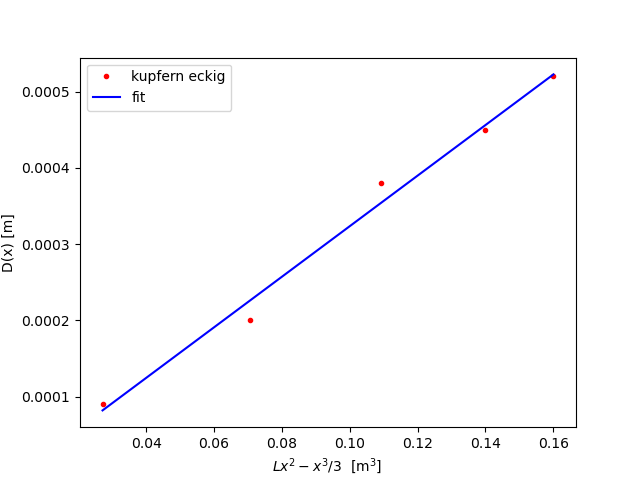
\includegraphics{keb.png}
    \captionof{figure}{Biegung eines kupfernen, eckigen Stabes mit zugehöriger Ausgleichsrechnung, bei beidseitiger Einspannung links vom Aufhängungspunkt.}
\end{figure}

\begin{figure}[H]
    \centering
    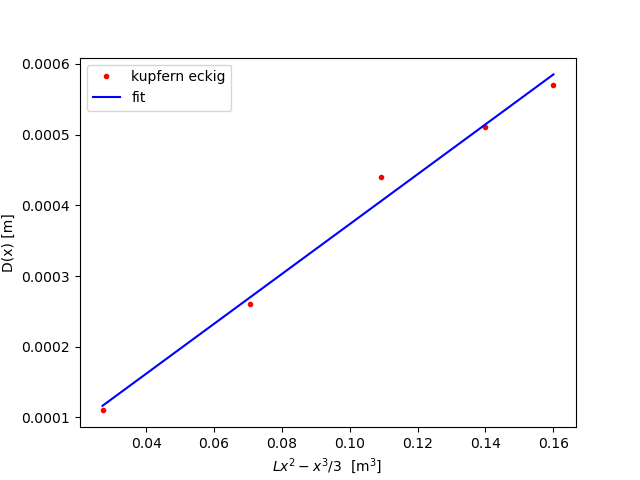
\includegraphics{keb2.png}
    \captionof{figure}{Biegung eines kupfernen, eckigen Stabes mit zugehöriger Ausgleichsrechnung, bei beidseitiger Einspannung rechts vom Aufhängungspunkt.}
\end{figure}

\begin{figure}[H]
    \centering
    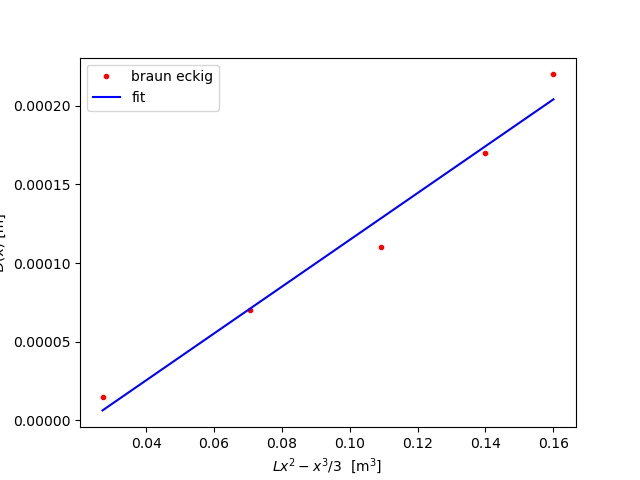
\includegraphics{beb.png}
    \captionof{figure}{Biegung eines braunen, eckigen Stabes mit zugehöriger Ausgleichsrechnung, bei beidseitiger Einspannung links vom Aufhängungspunkt.}
\end{figure}

\begin{figure}[H]
    \centering
    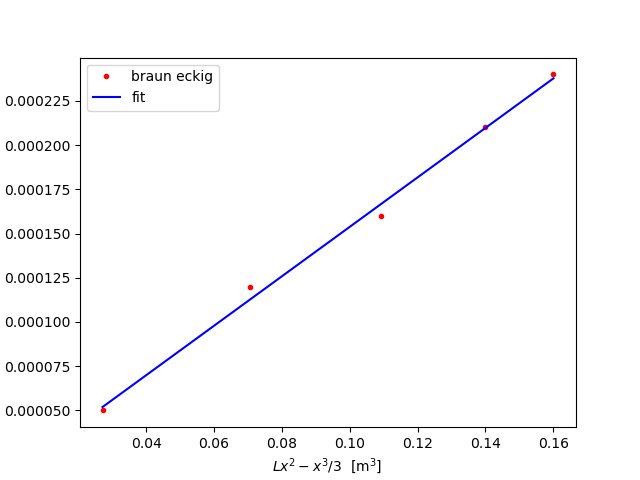
\includegraphics{beb2.png}
    \captionof{figure}{Biegung eines kupfernen, eckigen Stabes mit zugehöriger Ausgleichsrechnung, bei beidseitiger Einspannung rechts vom Aufhängungspunkt.}
\end{figure}

Die Ausgleichsrechnungen liefern folgende Steigungen:

\begin{align*}
    a_{Kupfer, links} = (3.3\pm 0.21) \frac{10^{-3}}{m^2}\\
    a_{Kupfer, rechts} = (3.5\pm 0.21) \frac{10^{-3}}{m^2}\\
    a_{braun, links} = (1.5\pm 0.14) \frac{10^{-3}}{m^2}\\
    a_{braun, rechts} = (1.4\pm 0.06) \frac{10^{-3}}{m^2}\\
\end{align*}

Mit diesen Steigungen können anschließend die Elastizitätsmodule berechnet werden. Dafür wird die folgende Gleichung benötigt:

\begin{displaymath}
    E = \frac{m*g}{48*I*a}
\end{displaymath}

Die angehängte Masse beträgt hier bei allen Gewichten 2.3408kg. Das Flächenträgheitsmoment ist das gleich wie bei vorherigen Rechnungen mit den eckigen Stäben. Dabei entstehen folgende Werte für die Elastizitätsmodule:

\begin{align*}
    E_{Kupfer, links} = (380\pm 40)GPa\\
    E_{Kupfer, rechts} = (410\pm 18)GPa\\
    E_{braun, links} = (174\pm 11)GPa\\
    E_{braun, rechts} = (164\pm 10)GPa\\
\end{align*}

\subsection{runde Stäbe, beidseitige Einspannung}

Zur Bestimmung dieser Elastizitätsmodule ist das Vorgehen sehr ähnlich dem Vorherigen. Die Werte für die Diagramme stammen allerdings aus \ref{tab:3} und \ref{tab:4}. Die Diagramme sehen diesmal folgendermaßen aus:

\begin{figure}[H]
    \centering
    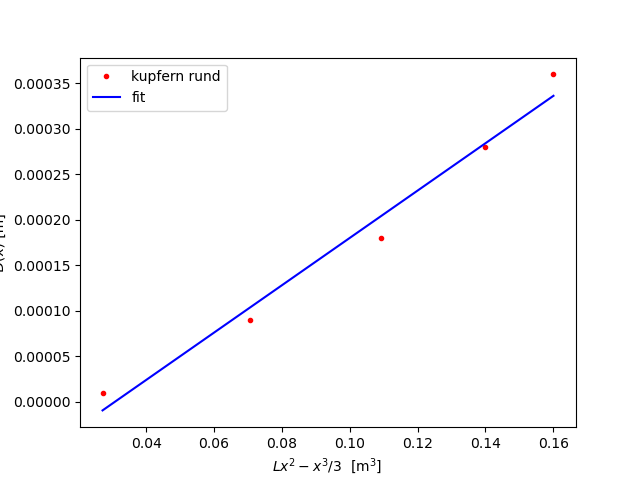
\includegraphics{krb.png}
    \captionof{figure}{Biegung eines kupfernen, runden Stabes mit zugehöriger Ausgleichsrechnung, bei beidseitiger Einspannung links vom Aufhängungspunkt.}
\end{figure}

\begin{figure}[H]
    \centering
    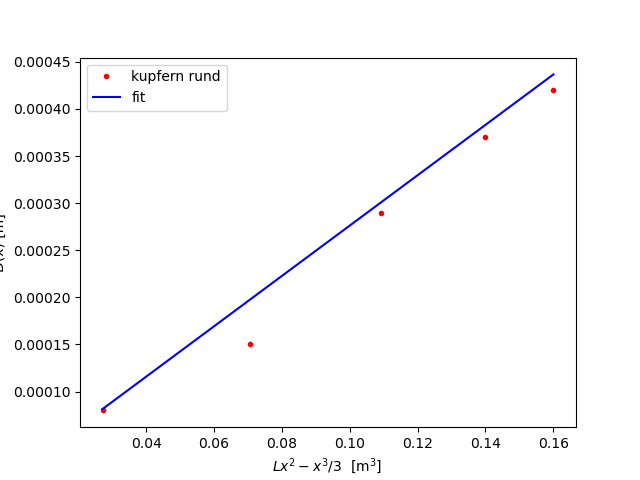
\includegraphics{krb2.png}
    \captionof{figure}{Biegung eines kupfernen, runden Stabes mit zugehöriger Ausgleichsrechnung, bei beidseitiger Einspannung rechts vom Aufhängungspunkt.}
\end{figure}

\begin{figure}[H]
    \centering
    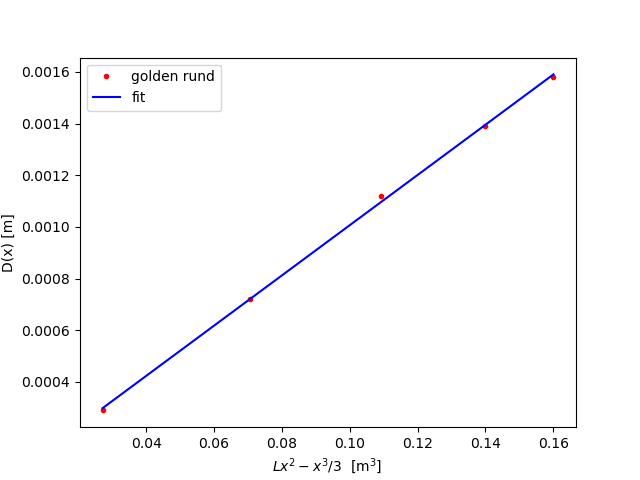
\includegraphics{grb.png}
    \captionof{figure}{Biegung eines goldenen, runden Stabes mit zugehöriger Ausgleichsrechnung, bei beidseitiger Einspannung links vom Aufhängungspunkt.}
\end{figure}

\begin{figure}[H]
    \centering
    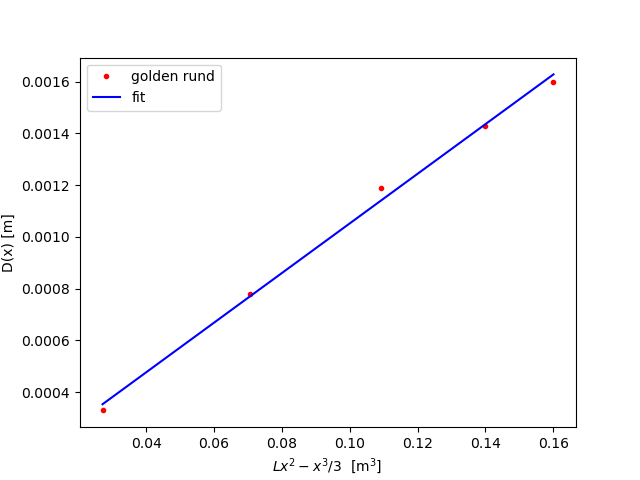
\includegraphics{grb2.png}
    \captionof{figure}{Biegung eines goldenen, runden Stabes mit zugehöriger Ausgleichsrechnung, bei beidseitiger Einspannung rechts vom Aufhängungspunkt.}
\end{figure}

Die Ausgleichsrechnungen liefern folgende Steigungen:

\begin{align*}
    a_{kupfer, links} = (2.6\pm 0.22) \frac{10^{-3}}{m^2}\\
    a_{kupfer, rechts} = (2.7\pm 0.19) \frac{10^{-3}}{m^2}\\
    a_{golden, links} = (9.7\pm 0.15) \frac{10^{-3}}{m^2}\\
    a_{golden, rechts} = (9.6\pm 0.34) \frac{10^{-3}}{m^2}\\
\end{align*}

Mit diesen Steigungen können anschließend die Elastizitätsmodule berechnet werden. Dafür wird die folgende Gleichung benötigt:

\begin{displaymath}
    E = \frac{m*g}{48*I*a}
\end{displaymath}

Die am kupferfarbenen Stab angehängte Masse beträgt 1,7294kg. Die am goldenen Stab angehängte Masse beträgt 2.3408kg. Das Flächenträgheitsmoment ist das gleiche wie bei der vorherigen Rechnung mit runden Stäben. Bei der Rechnung ergeben sich diese Elastizitätsmodule: 

\begin{align*}
    E_{kupfer, links} = (277\pm 23)GPa\\
    E_{kupfer, rechts} = (267\pm 19)GPa\\
    E_{golden, links} = (100.5\pm 1.6)GPa\\
    E_{golden, rechts} = (102\pm 4)GPa\\
\end{align*}

\subsection{Materialbestimmung durch Dichte}

\subsubsection{brauner, eckiger Stab}

Das Gewicht dieses Stabes beträgt 0.4546kg. Er hat einen quadratischen Querschnitt mit Kantenlänge a=1cm. Dazu ist der Stab 59.4cm lang. Daraus ergibt sich eine Dichte von: 7653.20$\frac{kg}{m^3}$.
Der Farbe und der dichte nach zu urteilen handelt es sich bei dem Material dieses Stabes um Stahl.

\subsubsection{kupferner, eckiger Stab}

Das Gewicht dieses Stabes beträgt 0.5359kg. Er hat einen quadratischen Querschnitt mit Kantenlänge a=1cm. Dazu ist der Stab 60.2cm lang. Daraus ergibt sich eine Dichte von: 8902.00$\frac{kg}{m^3}$.
Der Farbe und der dichte nach zu urteilen handelt es sich bei dem Material dieses Stabes um Kupfer.

\subsubsection{kupferner, runder Stab}

Das Gewicht dieses Stabes beträgt 0.4168kg. Er hat einen runden Querschnitt mit Durchmesser r=1cm. Dazu ist der Stab 60.2cm lang. Daraus ergibt sich eine Dichte von: 8811.84$\frac{kg}{m^3}$.
Der Farbe und der dichte nach zu urteilen handelt es sich bei dem Material dieses Stabes um Kupfer.

\subsubsection{goldener, runder Stab}

Das Gewicht dieses Stabes beträgt 0.394kg. Er hat einen runden Querschnitt mit Durchmesser r=1cm. Dazu ist der Stab 60.2cm lang. Daraus ergibt sich eine Dichte von: 8329.81$\frac{kg}{m^3}$.
Der Farbe und der dichte nach zu urteilen handelt es sich bei dem Material dieses Stabes um Messing.

\section{Diskussion}

Zu Beginn der Diskussion sind hier nocheinmal alle Elastizitätsmodule gebündelt aufgeführt:

\begin{align*}
    E_{braun, eckig} = (223\pm 9) GPa \\
    E_{kupfern, eckig} = (122\pm 4) GPa \\
    E_{kupfern, rund} = (146.5\pm 2.6) GPa \\
    E_{golden, rund} = (89\pm 17) GPa \\
    E_{kupfern, eckig, links} = (380\pm 40)GPa\\
    E_{kupfern, eckig, rechts} = (410\pm 18)GPa\\
    E_{braun, eckig, links} = (174\pm 11)GPa\\
    E_{braun, eckig, rechts} = (164\pm 10)GPa\\
    E_{kupfern, rund, links} = (277\pm 23)GPa\\
    E_{kupfern, rund, rechts} = (267\pm 19)GPa\\
    E_{golden, rund, links} = (100.5\pm 1.6)GPa\\
    E_{golden, rund, rechts} = (102\pm 4)GPa\\
\end{align*}

\section{Literatur}

\hyperlink{Dichte}{https://de.wikibooks.org/wiki/Tabellensammlung_Chemie/_Dichte_fester_Stoffe}

\section{Messwerte}

\begin{minipage}{\linewidth}
    \begin{table}[H]
        \centering
    \captionof{table}{brauner, eckiger Stab}
    \begin{tabular}{lll}
        \toprule
        x [cm] & D(x) (einseitig) [mm] & D(x) (beidseitig) [mm] \\
        \midrule
        3  & 0.03 & 0.015 \\
        8  & 0.14 & 0.07  \\
        13 & 0.32 & 0.11  \\
        18 & 0.59 & 0.17  \\
        23 & 0.85 & 0.22  \\
        32 & 1.46 & 0.24  \\
        37 & 1.72 & 0.21  \\
        42 & 1.88 & 0.16  \\
        47 & 2.30 & 0.12  \\
        52 & 3.00 & 0.05  \\
        \bottomrule   
    \end{tabular}
    
    \label{tab:1}
\end{table}
\end{minipage}


\begin{minipage}{\linewidth}
    \begin{table}[H]
        \centering
    \captionof{table}{kupferner, eckiger Stab}
    \begin{tabular}{lll}
        \toprule
        x [cm] & D(x) (einseitig) [mm] & D(x) (beidseitig) [mm] \\
        \midrule
        3  & 0.04 & 0.09 \\
        8  & 0.21 & 0.20 \\
        13 & 0.49 & 0.38 \\
        18 & 0.93 & 0.45 \\
        23 & 1.29 & 0.52 \\
        32 & 2.28 & 0.57 \\
        37 & 2.62 & 0.51 \\
        42 & 3.45 & 0.44 \\
        47 & 4.35 & 0.26 \\
        52 & 5.36 & 0.11 \\
        \bottomrule   
    \end{tabular}
    
    \label{tab:2}
\end{table}
\end{minipage}

\begin{minipage}{\linewidth}
    \begin{table}[H]
        \centering
    \captionof{table}{kupferner, runder Stab}
    \begin{tabular}{lll}
        \toprule
        x [cm] & D(x) (einseitig) [mm] & x2 [cm] & D(x) (beidseitig) [mm] \\
        \midrule
        3  & 0.01 & 3  & 0.01 \\ 
        8  & 0.07 & 8  & 0.09 \\ 
        13 & 0.17 & 13 & 0.18 \\ 
        18 & 0.32 & 18 & 0.28 \\ 
        23 & 0.48 & 23 & 0.36 \\ 
        28 & 0.67 & 32 & 0.42 \\ 
        33 & 0.82 & 37 & 0.37 \\ 
        38 & 1.02 & 42 & 0.29 \\ 
        43 & 1.32 & 47 & 0.15 \\ 
        48 & 1.49 & 52 & 0.08 \\ 
        \bottomrule   
    \end{tabular}
    
    \label{tab:3}
\end{table}
\end{minipage}

\begin{minipage}{\linewidth}
    \begin{table}[H]
        \centering
    \captionof{table}{goldener, runder Stab}
    \begin{tabular}{lll}
        \toprule
        x [cm] & D(x) (einseitig) [mm] & x2 [cm] & D(x) (beidseitig) [mm] \\
        \midrule
        3  & 0.06 & 3  & 0.29 \\ 
        8  & 0.26 & 8  & 0.72 \\ 
        13 & 0.61 & 13 & 1.12 \\ 
        18 & 1.10 & 18 & 1.39 \\ 
        23 & 1.70 & 23 & 1.58 \\ 
        28 & 2.46 & 32 & 1.60 \\ 
        33 & 3.1  & 37 & 1.43 \\ 
        38 & 3.8  & 42 & 1.19 \\ 
        43 & 4.75 & 47 & 0.78 \\ 
        48 & 5.37 & 52 & 0.33 \\ 
        \bottomrule   
    \end{tabular}
    
    \label{tab:4}
\end{table}
\end{minipage}